\begin{frame}
    \frametitle{Columnar}

    Las bases de datos orientadas a columnas almacenan datos verticalmente por columnas en lugar de horizontalmente por filas, permitiendo un acceso más eficiente a datos específicos.
    
    \begin{center}
        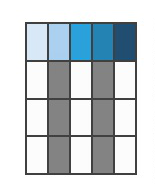
\includegraphics[width=0.3\textwidth]{diagramas/Columnar.png}
    \end{center}
\end{frame}


\begin{frame}
    \frametitle{Columnar - Ventajas}

    \begin{itemize}
        \item  Mayor eficiencia en consultas sobre columnas específicas.  
        \item  Convenientes para análisis de grandes volúmenes de datos.  
        \item  Adecuadas para aplicaciones de business intelligence y análisis predictivo.
    \end{itemize}
\end{frame}

\begin{frame}
    \frametitle{Columnar - Desventajas}
    \begin{itemize}
        \item  Operaciones de escritura más lentas debido a la reorganización de datos en columnas específicas.  
        \item  Posibles desafíos en entornos con datos altamente transaccionales.
    \end{itemize}
\end{frame}

\begin{frame}
    \frametitle{Columnar - Ejemplos}

    Algunos ejemplos de bases de datos columnares son: 
    
    \begin{itemize}
        \item \textbf{Apache Cassandra}\\
        Aunque es principalmente una base de datos de clave-valor, Cassandra utiliza un modelo de almacenamiento columnar para mejorar el rendimiento de ciertas consultas.  
        \item \textbf{Apache HBase}\\
        HBase es una base de datos de columnas distribuida, que almacena datos de forma columnar y permite un acceso eficiente a través de claves de fila.   
        \item \textbf{ClickHouse}\\
        ClickHouse es una base de datos de análisis columnar de código abierto diseñada para consultas analíticas de alto rendimiento en grandes conjuntos de datos.
    \end{itemize}
\end{frame}